\documentclass[12pt,a4paper]{amsart}
%\usepackage[norsk]{babel}
\usepackage[english]{babel}
\usepackage[utf8]{inputenc}
%\usepackage[fleqn]{amsmath}
\usepackage{amsmath}
\usepackage[T1]{fontenc}
\usepackage{mathtools}
\usepackage{graphicx}
\usepackage{subcaption}
\usepackage{verbatim}
\usepackage{listings}
\usepackage{scalerel}
\usepackage{fixltx2e}
\usepackage{amssymb}
\usepackage{siunitx}
\usepackage{xfrac}
\usepackage{enumitem}
\usepackage{hyperref}
\usepackage{float}
\usepackage{bbold}
\usepackage{physics}
\usepackage[ampersand]{easylist}
\usepackage{subcaption}
\usepackage{wrapfig}
\usepackage{algorithmicx}
\usepackage{csquotes}
\usepackage{xcolor}

%%For visualizations of table
\usepackage{multirow}
\usepackage{arydshln}
\usepackage{booktabs}

\usepackage[english]{babel}\addto\captionsenglish  
{\renewcommand{\bibname}{References}}  
\usepackage[backend=bibtex,style=phys]{biblatex}  %backend=biber is 'better'  
%\usepackage[backend=biber]{biblatex}
%\usepackage{apacite}
\addbibresource{cosmic_rays_bibliography.bib}

\usepackage[margin=1.5in]{geometry}
\newcommand{\scalel}{\scaleleft{<}}
\newcommand{\scaler}{\scaleright{>}}

%% physics packages
\usepackage{physics}
\usepackage[compat=1.1.0]{tikz-feynman}
\usepackage{feynmf}

% adjust the spacing around figure if pdf-file with white space:
\usepackage[font=small,skip=0pt]{caption}
%\usepackage[margin=1.4in]{geometry}
%\captionsetup[figure]{skip=-100pt}

% define colors for text
\definecolor{mygreen}{RGB}{28,172,0} % color values Red, Green, Blue
\definecolor{mylilas}{RGB}{170,55,241}
\definecolor{forestgreen}{rgb}{0.13, 0.55, 0.13}

% definitions of commands
\renewcommand{\thesection}{\arabic{section}}
\newcommand{\M}{\CMcal{M}}
\newcommand{\p}[1]{p_{#1}}  %p with one parameters such that \p1 = p_1, \p2 = p_2 etc.
\newcommand{\q}[2]{\ensuremath{p_{#1}\cdot p_{#2}}}  %p with two parameters such that \p12 = p_1\cdot p_2
\newcommand{\cmuplus}{c_V^2 + c_A^2}
\newcommand{\cmuminus}{c_V^2 - c_A^2}
\newcommand{\cbplus}{\tilde{c}_V^2 + \tilde{c}_A^2}
\newcommand{\cbminus}{\tilde{c}_V^2 - \tilde{c}_A^2}

% layout for sections, subsections and subsubsections
\usepackage{titlesec}
\renewcommand{\thesubsection}{\arabic{subsection}} % Arabic numerals for the subsections
\titleformat{\subsection}{\scshape\large\filcenter}{\arabic{section}.\thesubsection.}{1em}{}

\title[Charged particles study with PolarquEEEst]{Project 2: \\Study of cosmic charged particle events with the PolarquEEEst experiment\\
\small{\mdseries FYS5555 - Spring 2020}}
\date{\today}
\author[Christensen]{Elisabeth Christensen}

\begin{document}
\maketitle
\setcounter{section}{1}
\setcounter{subsection}{0}
\subsection{Cosmic rays}
The study of cosmic rays began in the beginning of the 20'th century, and was triggered by the fact that radiation was able to penetrate even those of the most isolating materials. Using electrometers, one could measure the intensity of radiation at different altitudes. In 1912, Victor Hess discovered~\cite{Hess1912} that the radiation increased with increasing altitudes, meaning that the radiation must originate beyond our atmosphere. He excluded the Sun as the primary source of this type of radiation, and concluded that it must come from more distant sources such as other galaxies. Now, the reason as to why we wish to know more about these cosmic rays is due to their astonishingly high energies. An example of this is the 'Oh-My-God' particle, measured by the Fly's Eye experiment~\cite{OhMyGodParticle}, which reached the Earth's surface with an energy of $3.2\cdot 10^{20}$eV, i.e. more than a billion times greater than what our most advanced accelerators to date can manage. This leaves us with the bigger questions to answer. Where do these particles come from and how did they reach such high energies?

Primary cosmic rays are essentially high-energetic protons and alpha particles originating from the Sun or beyond our Solar system. Models indicate that cosmic rays of energies up to $\sim 10^{15}$eV originate from the shock fronts of supernova remnants~\cite{Ellison1997}. The AGASA observatory, situated in Japan, measures the higher end of the energy spectrum, i.e. up to $10^{20}$eV, of cosmic rays entering our atmosphere. Another observatory, the Pierre Auger Observatory, published its first results of the highest-energy cosmic rays in 2007. The observatory has also assisted in finding the energy spectrum for cosmic rays above $\sim 10^{18}$eV~\cite{Auger2010}, and found that the flux was propotional to $E^{-\gamma}$, where $\gamma$ is approximately equal to 3. It also supported the theory that within the center of each galaxy resides a black hole with the capacity to accelerate particles to energies up to $10^{20}$eV.

Secondary cosmic rays are essentially particle showers occuring when the primary cosmic rays interact with particles within our atmosphere. Secondary cosmic rays typically consist of neutrons and charged mesons which subsequently can decay to muons and neutrinos reaching the Earth's surface. There are many experiments dedicated to use secondary cosmic particles in the search for knowledge. Some examples are the CLOUD experiment at CERN~\cite{cloud2000}, designed to measure the correlation between cosmic rays and cloud formation, te balloon-borne experiment TRACER~\cite{tracer2007} designed to observe cosmic-ray nuclei at high energies, and the ground-based Cherenkov Telescope Array (CTA) observatory~\cite{cta2011}, dedicated to find the origin and role of relativistiv cosmic particles through the study of high-energy gamma-rays reaching Earth.

\setcounter{section}{2}
\setcounter{subsection}{0}
\subsection{POLA detectors}
Particles can be detected in numerous ways depending on their charge and energy, some examples being the ionization chamber, the proportional counter and the Geiger-Müller counter. The Geiger-Müller counter was one of the first few devices to detect particles and consists simply of an air-tight cylinder tube containing a suitable gas and a suspended conducting wire with a positive voltage. When charged particles strike the gas they will interact with molecules within the gas creating electron-ion pairs. The electrons will be accelerated towards the conducting wire, i.e. the anode, whereas ions will be accelerated towards the cathode. The total eletron-ion pairs collected results in a measurable electric current. Another example is that of scintillators.

Scintillators are based on the principle of luminescense~\cite{knoll2000}. In other words, as passing radiation strikes a luminescent material it converts the kinetic energy of the charged particles to detectable light. Put simply, scintillators gather the information of the emitted photons in photomultiplier tubes which outputs a current of electrons based on the energy of the impinging photon.

\begin{comment}
The PolarquEEEst experiment~\cite{PolarquEEEst_first_results} consists in total of three POLA detectors, each with the aim to measure the intensity of incoming atmopheric radiation at a certain latitude. POLA-01 was placed upon an 18m long boat, known as \textit{Nanuq}, and was shipped from Isafjord, Iceland to Tromsø, Norway continuously taking measurements between the latitudes of $66^\circ-82^\circ$N. POLA-03 is situated in Bra, Italy at a latitude of $44^\circ 41'$N, while POLA-02 is situated in Nesodden, Norway at a latitude of $59^\circ 51'$N.  The two latter detectors were used as references. POLA-01 also performed measurements down to $35^\circ$ in Italy.
\end{comment}

Each of the POLA detectors consists of two floors of four plastic scintillators with the dimensions $20\times30\times1 \si{cm}^3$. The main purpose of a plastic scintillator is to emit photons within the energy range of any passing charged particle. Plastic scintillators can provide an extremely fast signal with a decay constant of about $2-3\si{ns}$ along with a high light output~\cite{leo1994}. Attached to each scintillator is a pair silicon photomultiplier (SiPM) tubes. Included are also eight front-end boards each dedicated to handle the SiPM signals separately, and trigger on events with a $10$ns resolution.

\setcounter{section}{3}
\setcounter{subsection}{0}
\subsection{Environmental conditions}
From figure~\ref{fig:indoortemp_POLA-01} we can see the variations in indoor temperature onboard the 18m long sailboat Nanuq containing the detector POLA-01, from 22'nd of July 2018 to 4'th of September 2018. Each point represents the average indoor temperature recorded per event over a time interval of 10 minutes. The corresponding indoor temperatures for POLA-02 and POLA-03 can be seen in figures~\ref{fig:indoortemp_POLA-02} and~\ref{fig:indoortemp_POLA-03}. Figure~\ref{fig:outdoortemp} shows the temperatures close to the electronics for each detector. The corresponding mean values and sample standard deviations of the temperatures can be seen in table~\ref{tab:temperatures}. Here, we see that the variations in temperature for POLA-01 are much greater than that for POLA-02 and POLA-03, which can be explained by the fact that it was subject to varying weather conditions while travelling between Isafjord, Iceland and Tromsø, Norway.

Figure~\ref{fig:pressure} shows the atmospheric pressure each detector is subject to. This is dependent on the surrounding temperature and the elevation above sea level. As can be seen for POLA-03, situated in Bra, Italy at an elevation of approximately 278m, resulting in a lower barometric pressure. 

\begin{table}[t]
\caption{Mean values of indoor, $\mu_{T, in}$, and outdoor, $\mu_{T, out}$, temperatures of each detector.}
\label{tab:temperatures}
\begin{tabular}{c|cc}
\hline
\hline
        & $\mu_{in} ({}^\circ \si{C})$ &$\mu_{out}({}^\circ \si{C})$ \\ \hline
POLA-01 & $25.39\pm 2.79$	& $23.75\pm 2.73$ \\
POLA-02 & $25.06\pm 0.14$    & $24.13\pm 0.12$ \\
POLA-03 & $33.37\pm 0.85$    & $34.67\pm 0.75$ \\
\hline \hline
\end{tabular}
\end{table}

\begin{figure}
\centering
	\begin{subfigure}[b]{\textwidth}
	\centering
		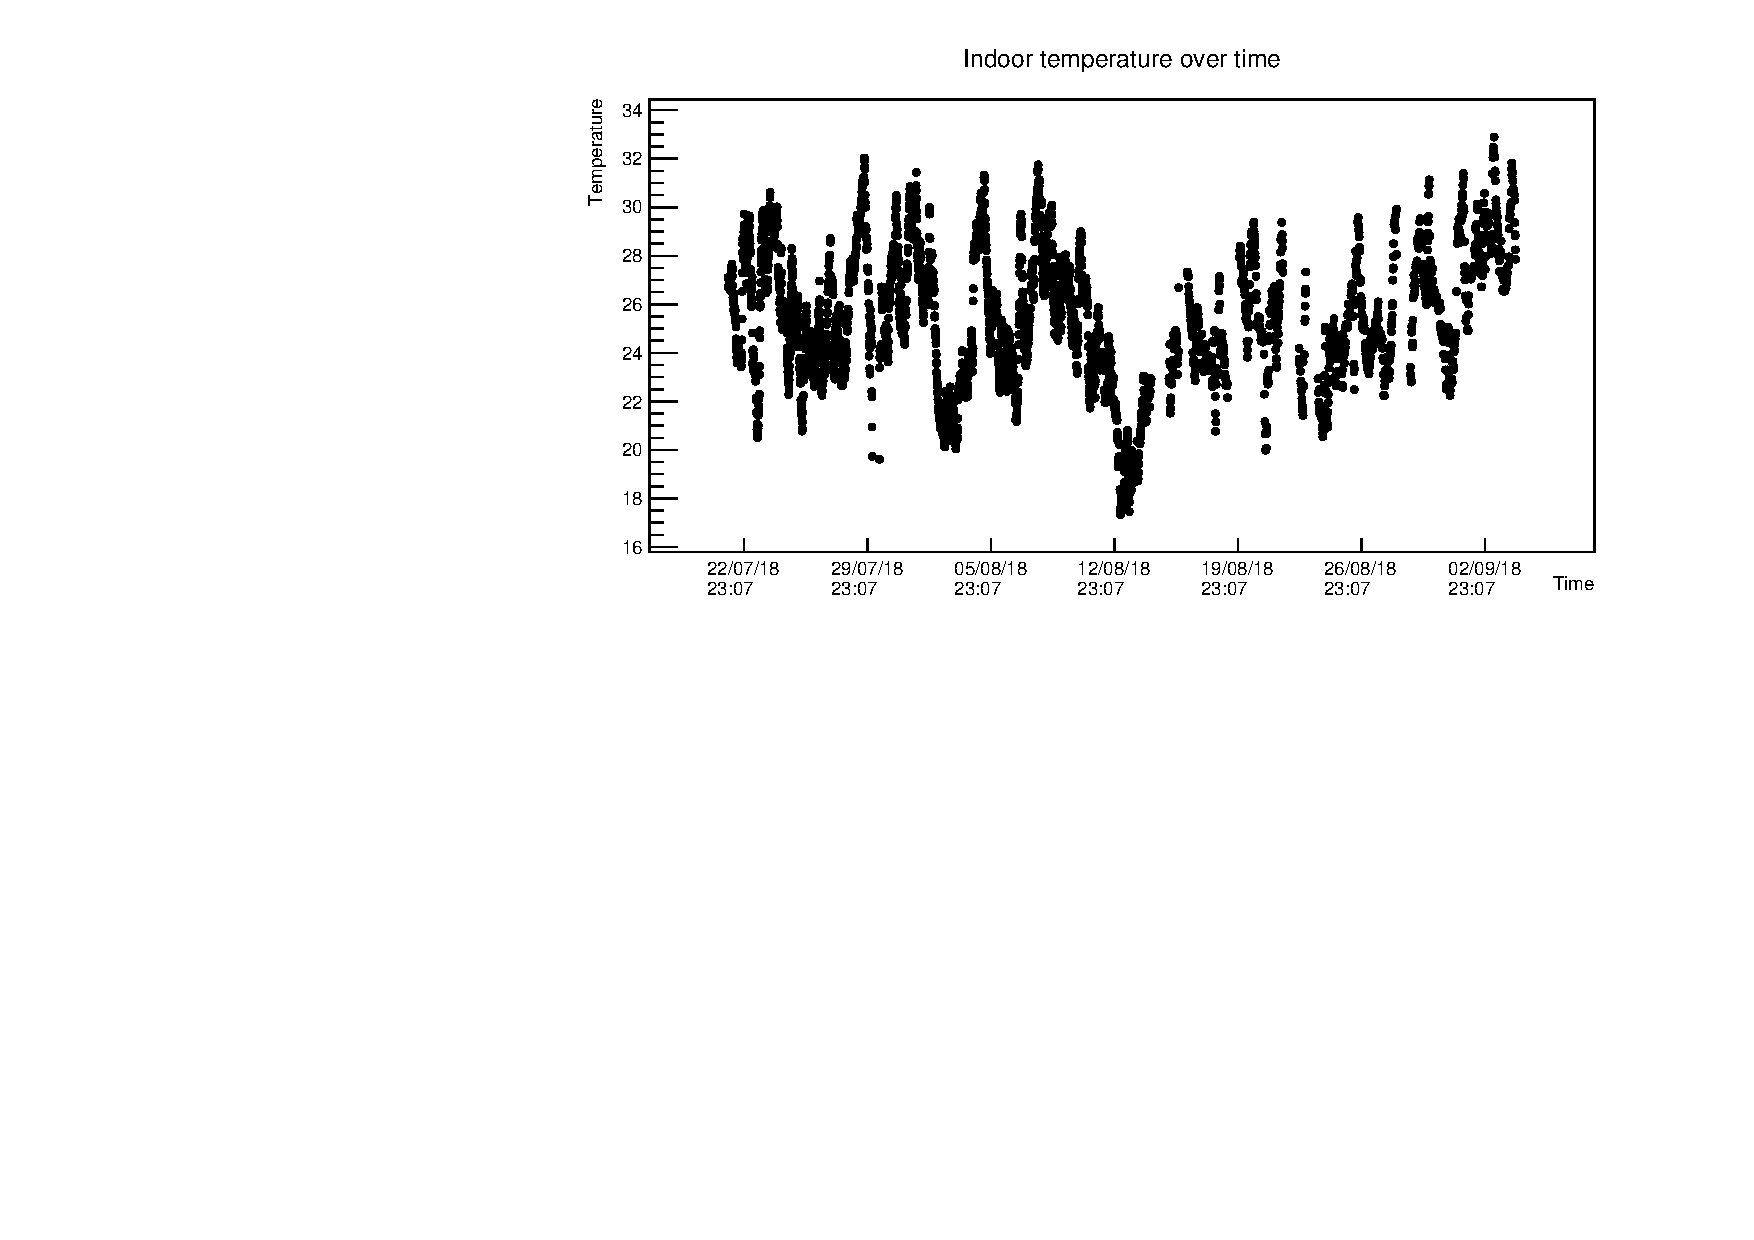
\includegraphics[width=\textwidth]{../data/plots/POLA-01/IndoorTemp_POLA-01.pdf}
		\caption{POLA-01}
		\label{fig:indoortemp_POLA-01}
	\end{subfigure}
	
	\begin{subfigure}[b]{0.6\textwidth}
	\centering
		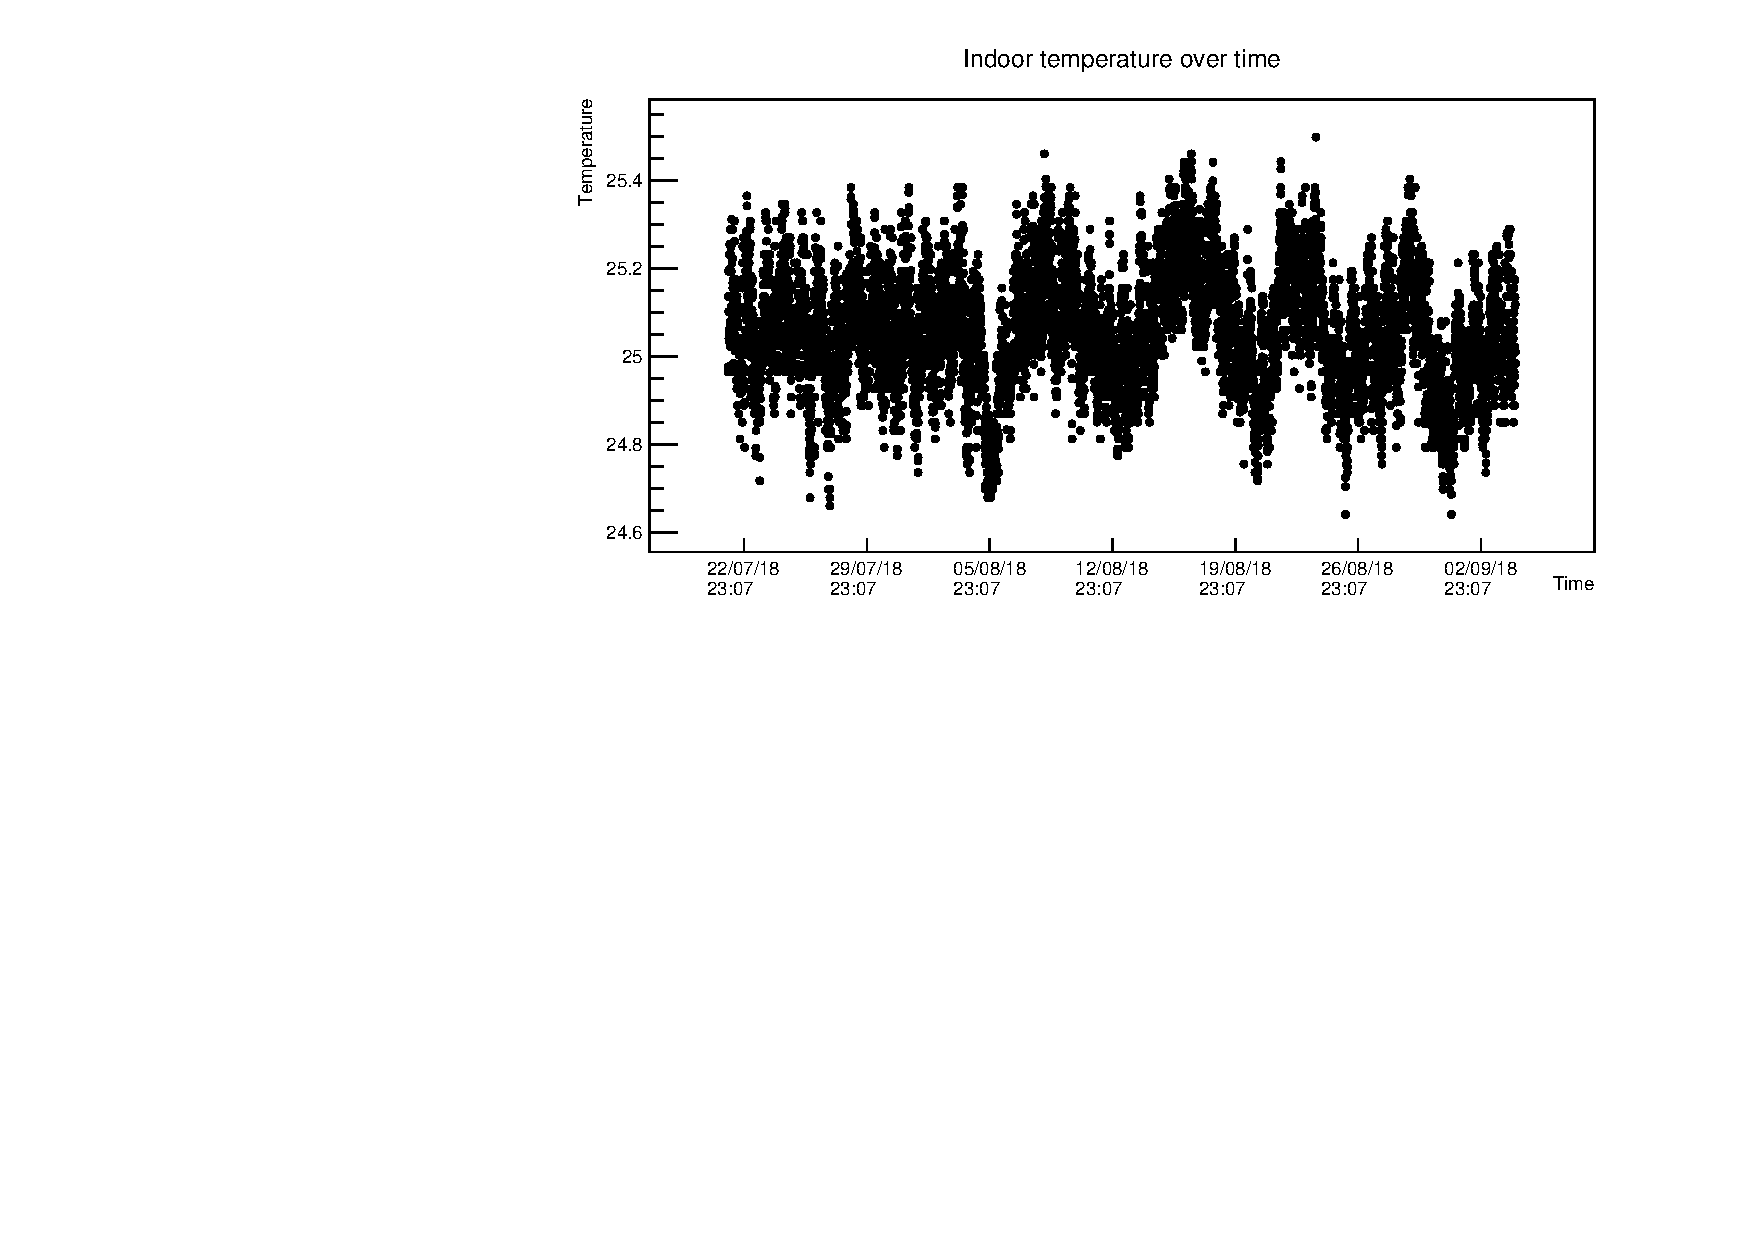
\includegraphics[width=\textwidth]{../data/plots/POLA-02/IndoorTemp_POLA-02.pdf}
		\caption{POLA-02}
		\label{fig:indoortemp_POLA-02}
	\end{subfigure}%
	\begin{subfigure}[b]{0.6\textwidth}
	\centering
		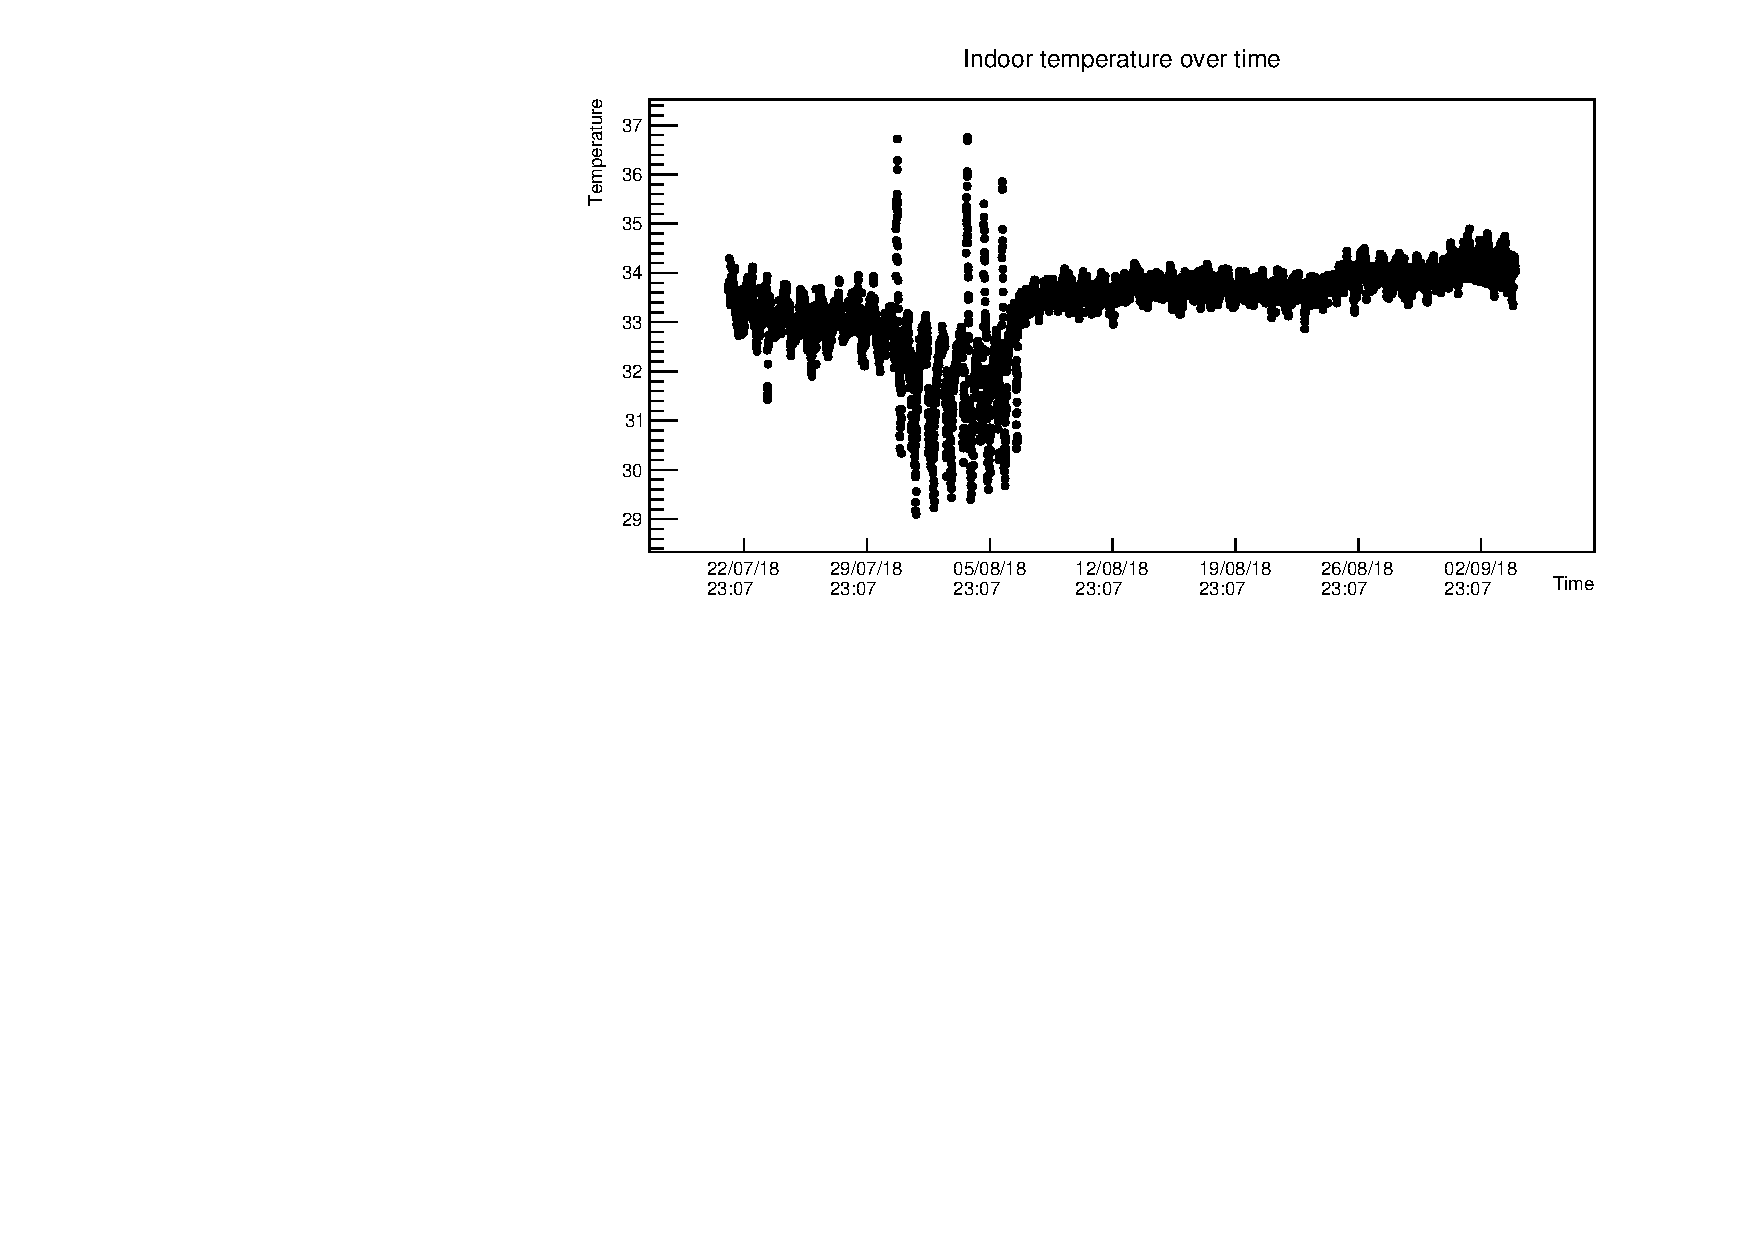
\includegraphics[width=\textwidth]{../data/plots/POLA-03/IndoorTemp_POLA-03.pdf}
		\caption{POLA-03}
		\label{fig:indoortemp_POLA-03}
	\end{subfigure}
	\caption{Indoor temperature as measured within each room containing the detectors.}
	\label{fig:indoortemp}
\end{figure}

\begin{figure}
\centering
	\begin{subfigure}[b]{\textwidth}
	\centering
		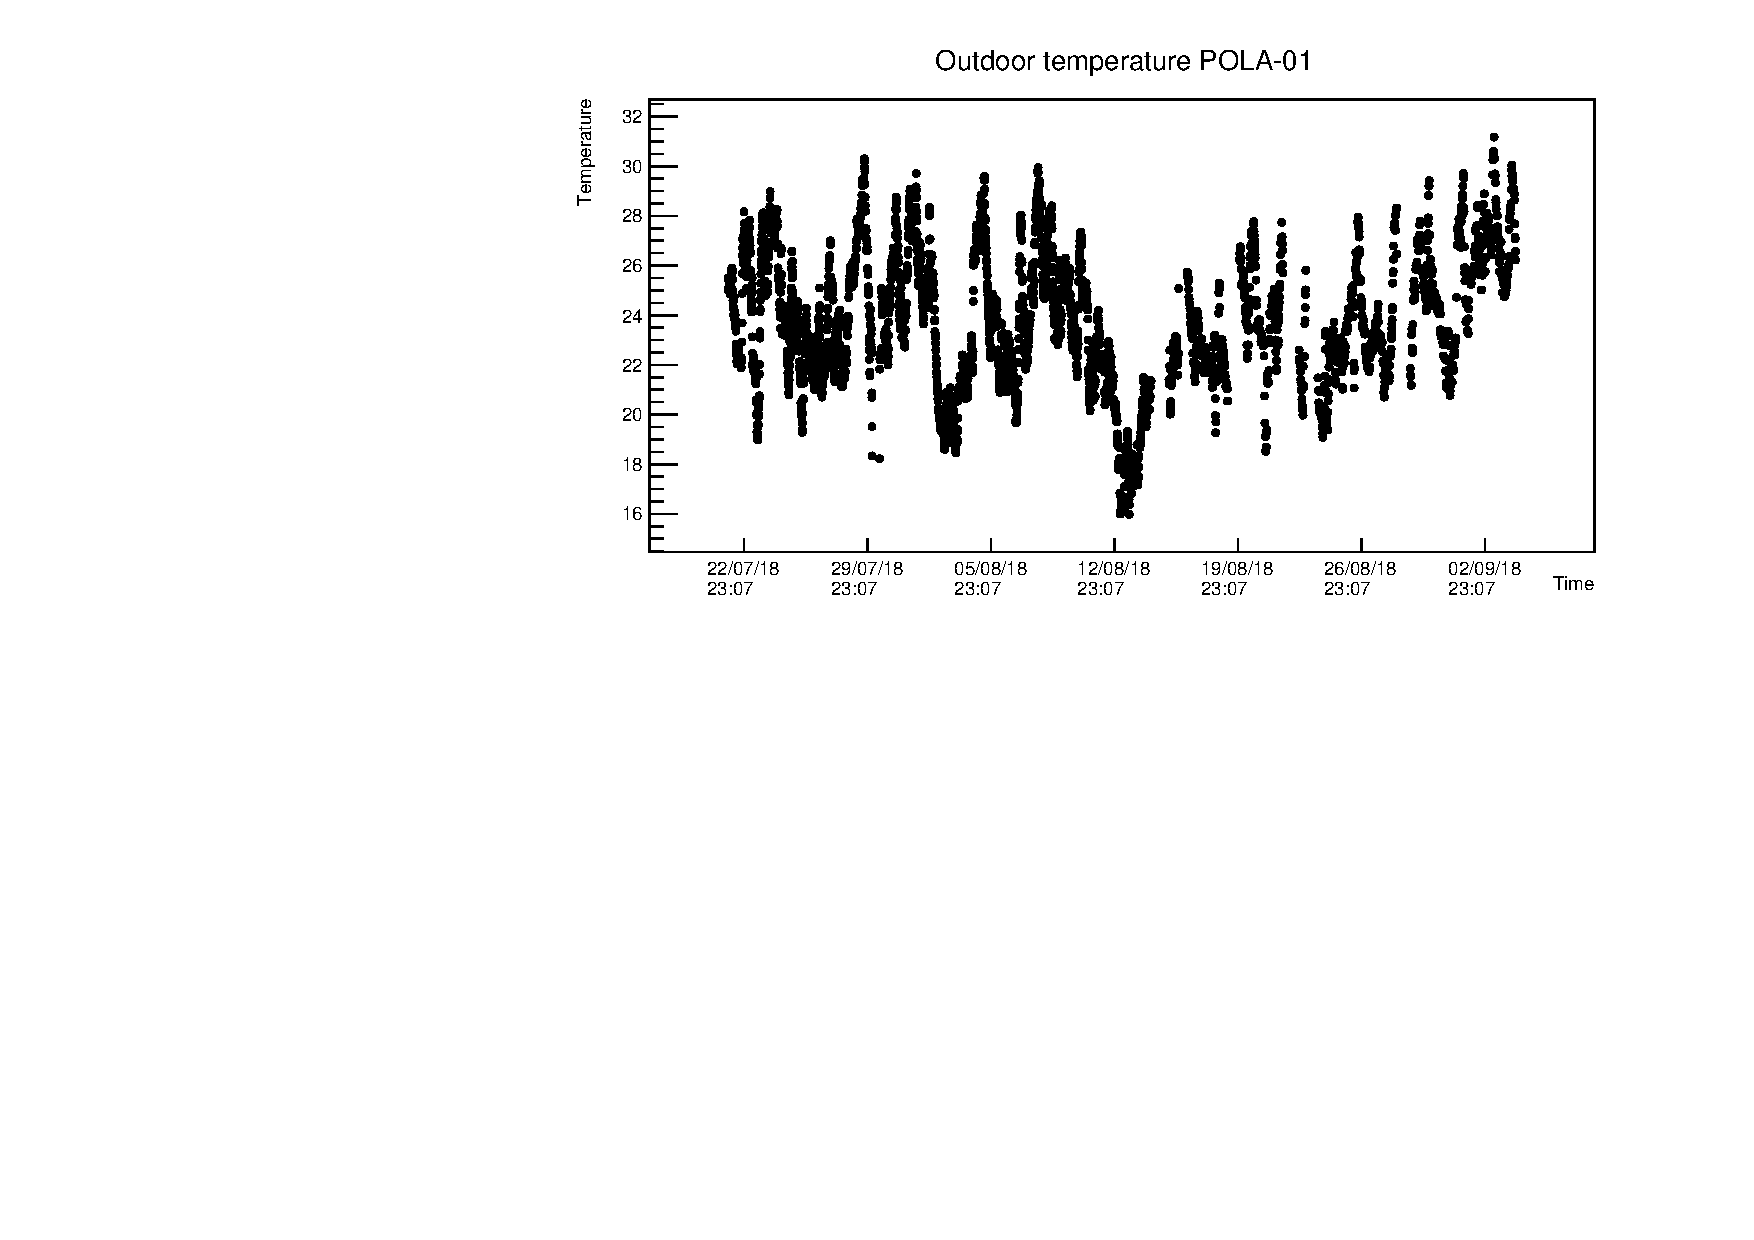
\includegraphics[width=\textwidth]{../data/plots/POLA-01/OutdoorTemp_POLA-01.pdf}
		\caption{POLA-01}
		\label{fig:outdoortemp_POLA-01}
	\end{subfigure}
	\begin{subfigure}[b]{0.6\textwidth}
	\centering
		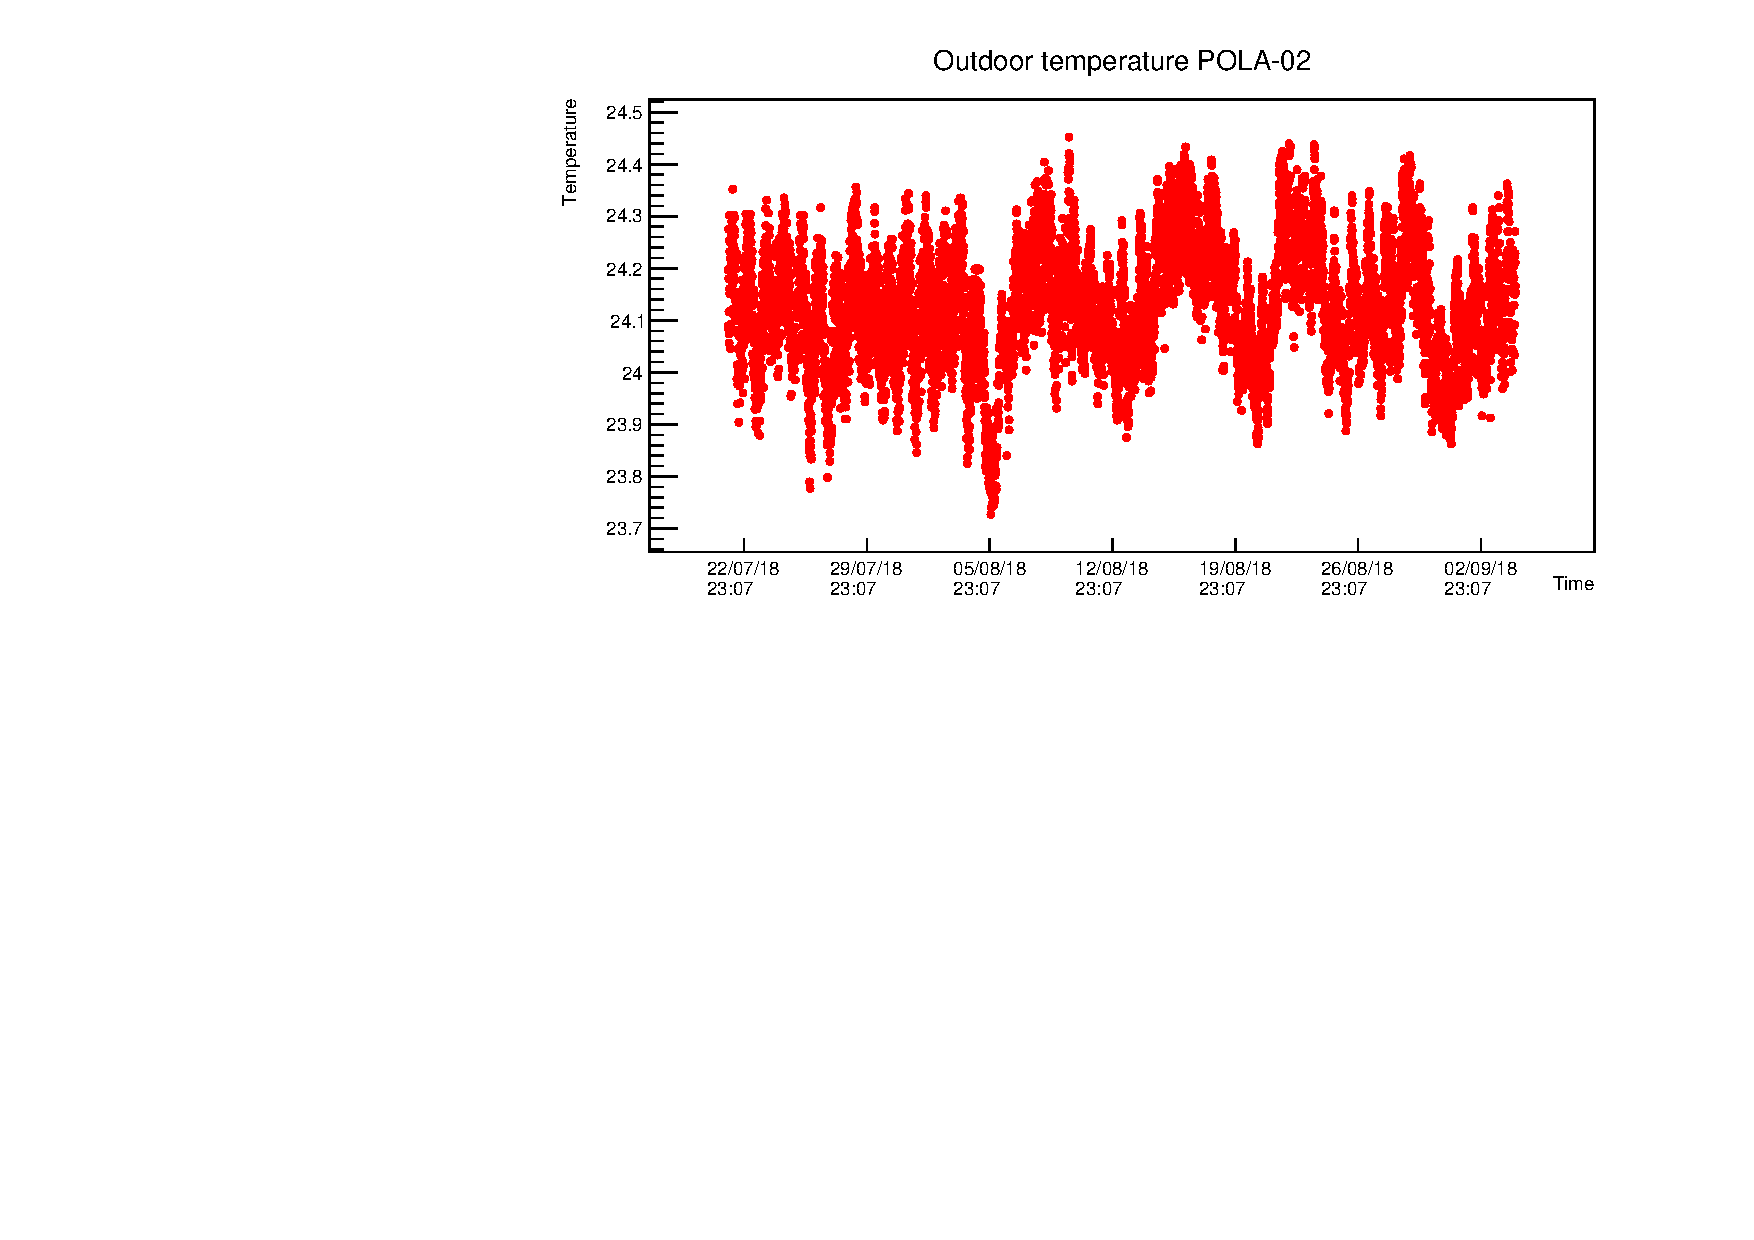
\includegraphics[width=\textwidth]{../data/plots/POLA-02/OutdoorTemp_POLA-02.pdf}
		\caption{POLA-02}
		\label{fig:outdoortemp_POLA-02}
	\end{subfigure}%
	\begin{subfigure}[b]{0.6\textwidth}
	\centering
		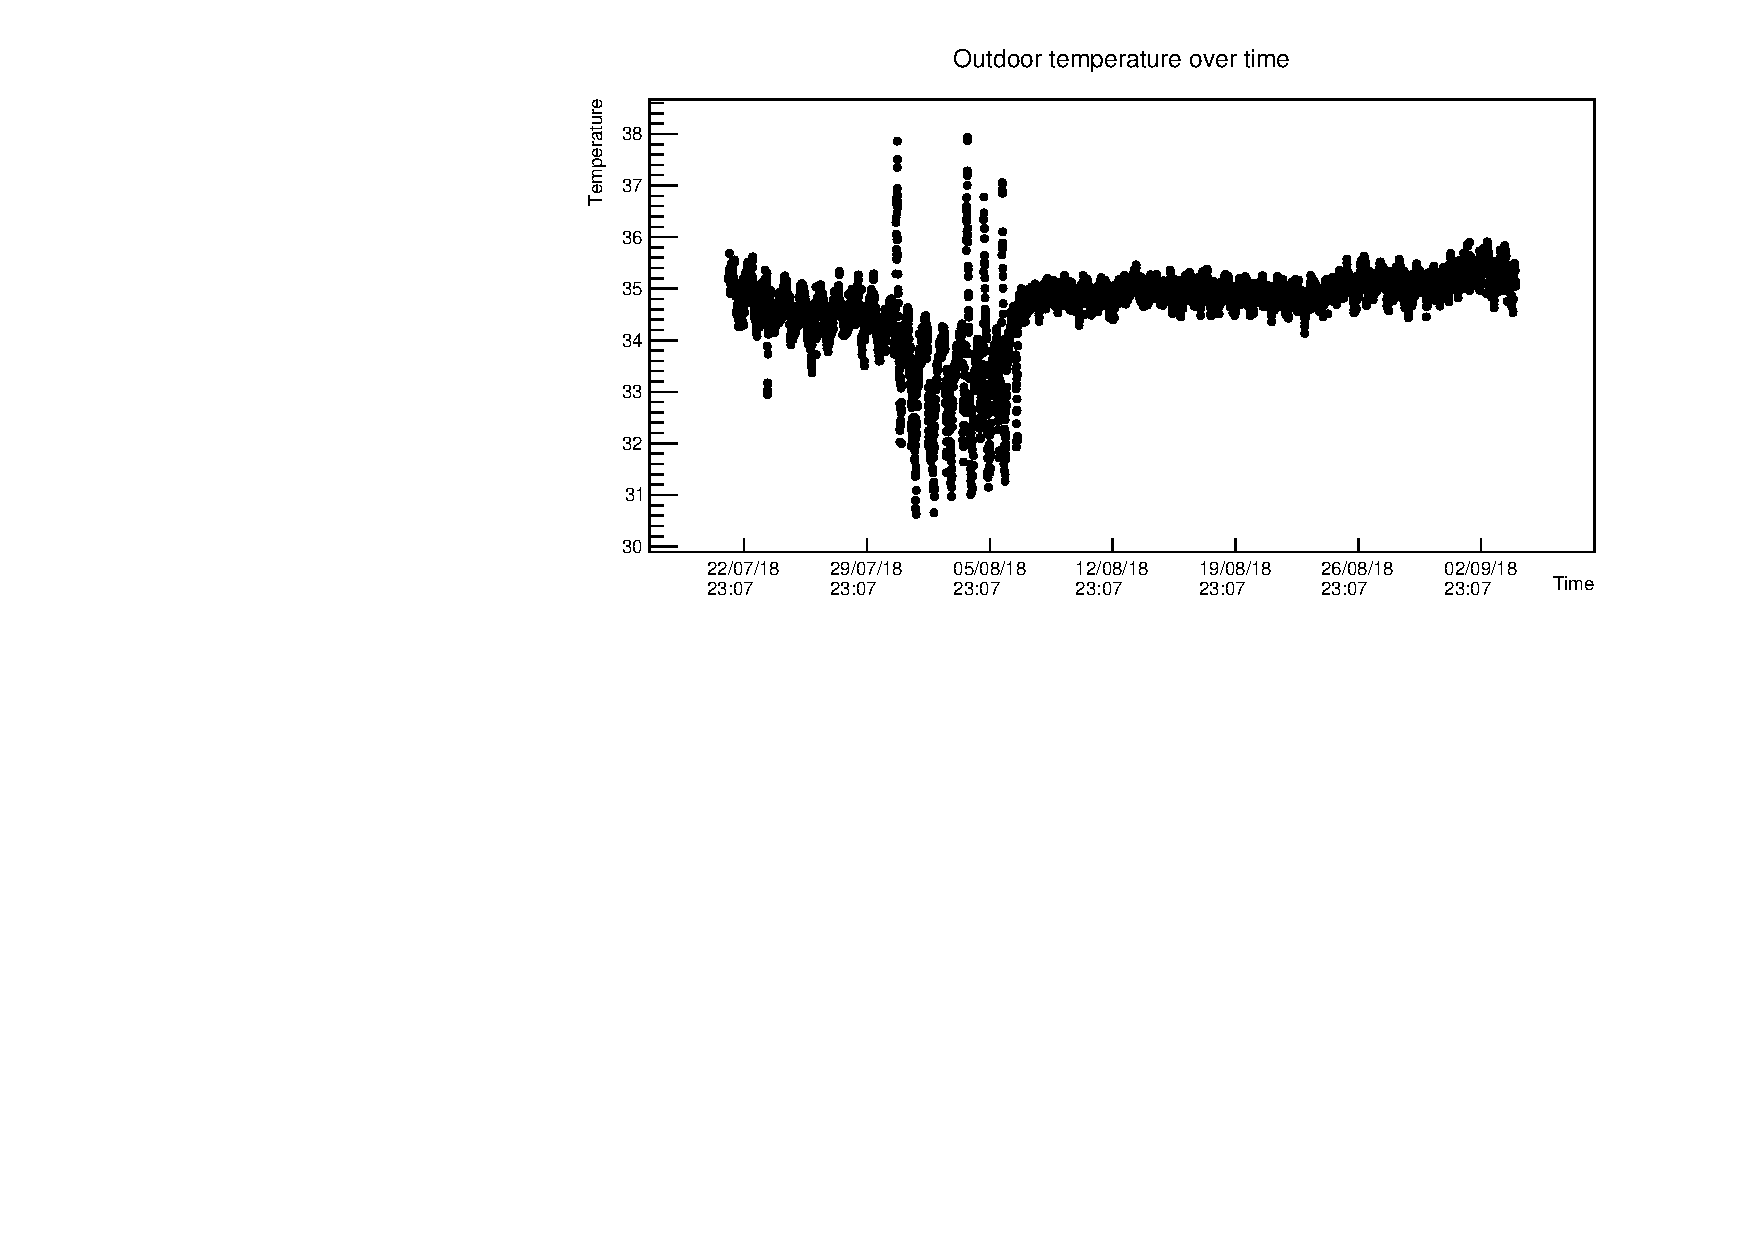
\includegraphics[width=\textwidth]{../data/plots/POLA-03/OutdoorTemp_POLA-03.pdf}
		\caption{POLA-03}
		\label{fig:outdoortemp_POLA-03}
	\end{subfigure}
	\caption{Outdoor temperature as measured close to the electronics of each detector.}
	\label{fig:outdoortemp}
\end{figure}

\begin{table}[t]
\begin{tabular}{c|c}
\hline\hline
        & $\mu_P$           \\ \hline
POLA-01 & $1012.62\pm 8.68$ \\
POLA-02 & $1008.56\pm 6.55$ \\
POLA-03 & $985.96\pm2.63$   \\
\hline \hline
\end{tabular}
\end{table}

\begin{figure}
\centering
	\begin{subfigure}[b]{\textwidth}
	\centering
		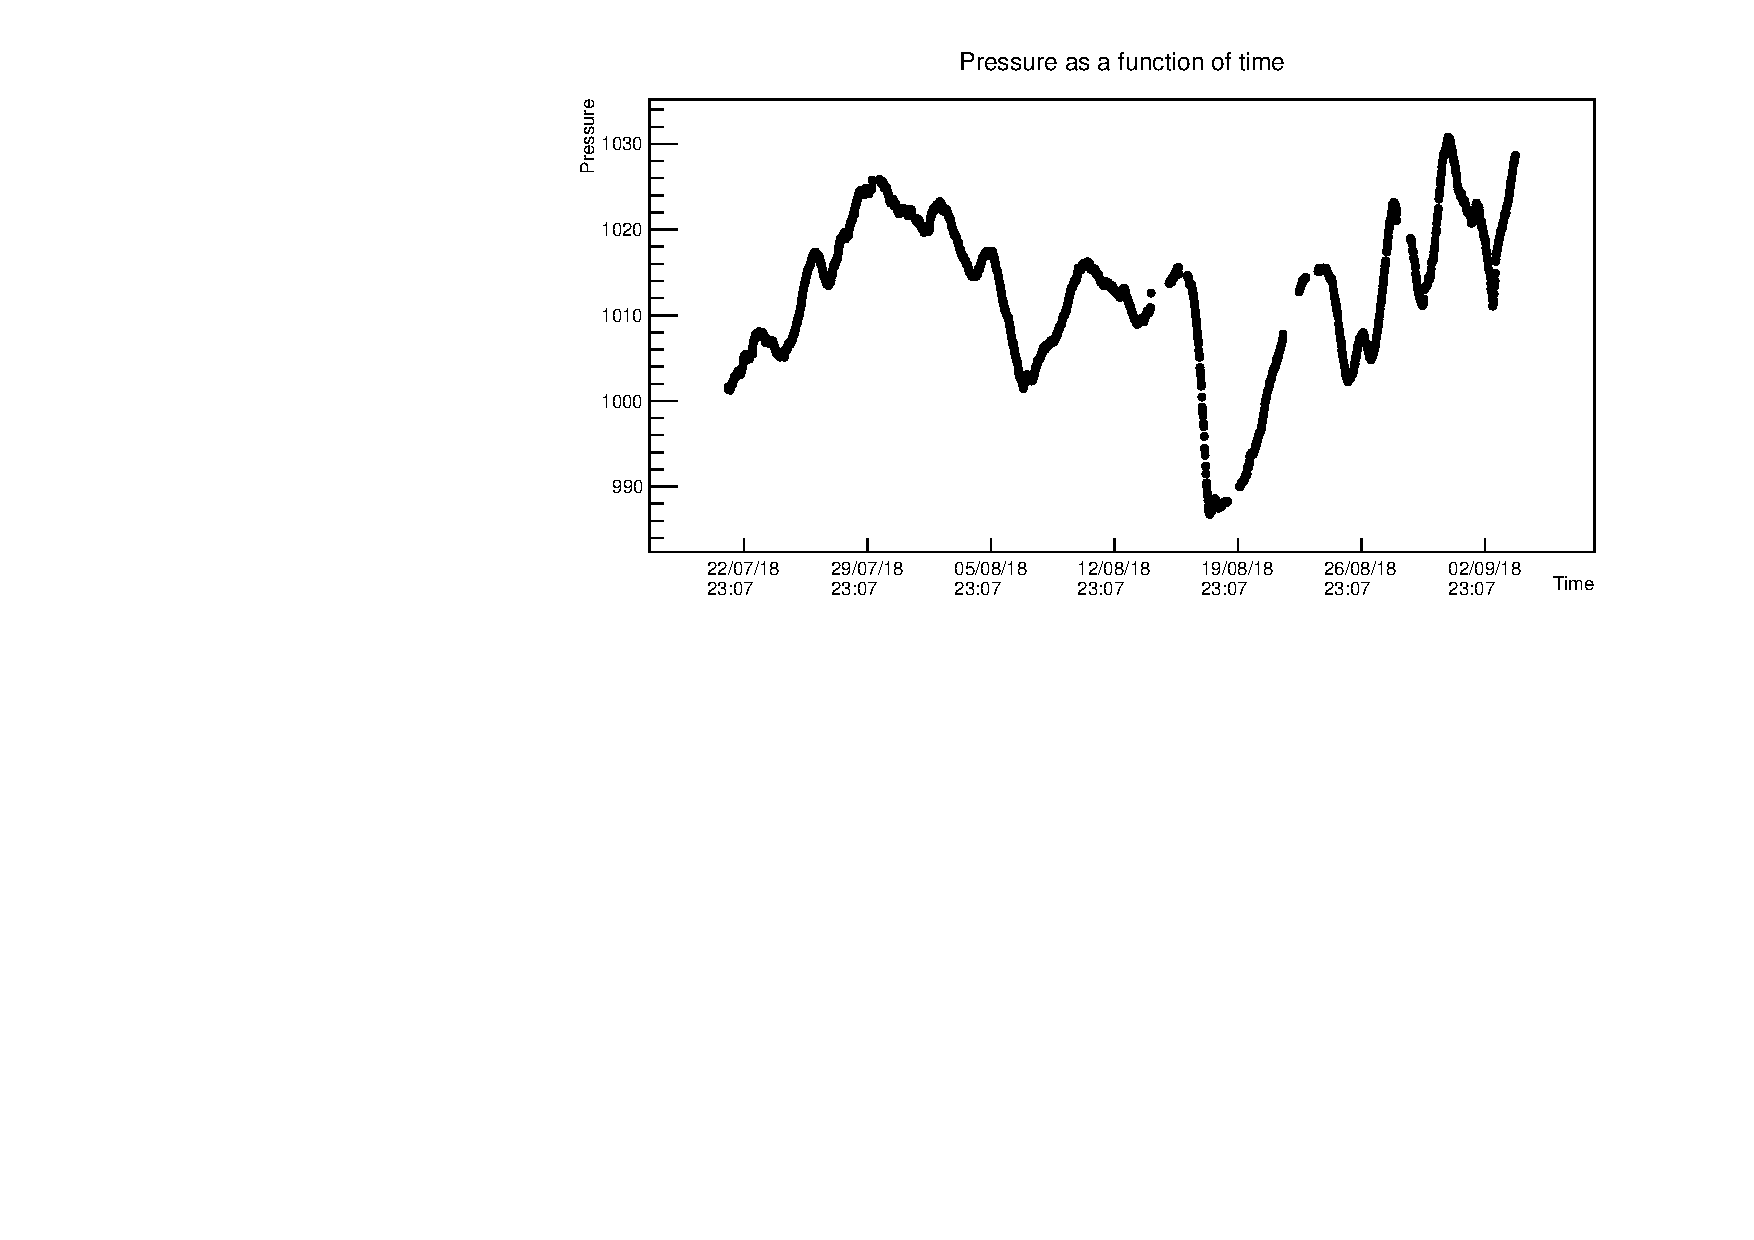
\includegraphics[width=\textwidth]{../data/plots/POLA-01/pressure_POLA-01.pdf}
		\caption{POLA-01}
		\label{fig:pressure_POLA-01}
	\end{subfigure}
	\begin{subfigure}[b]{0.6\textwidth}
	\centering
		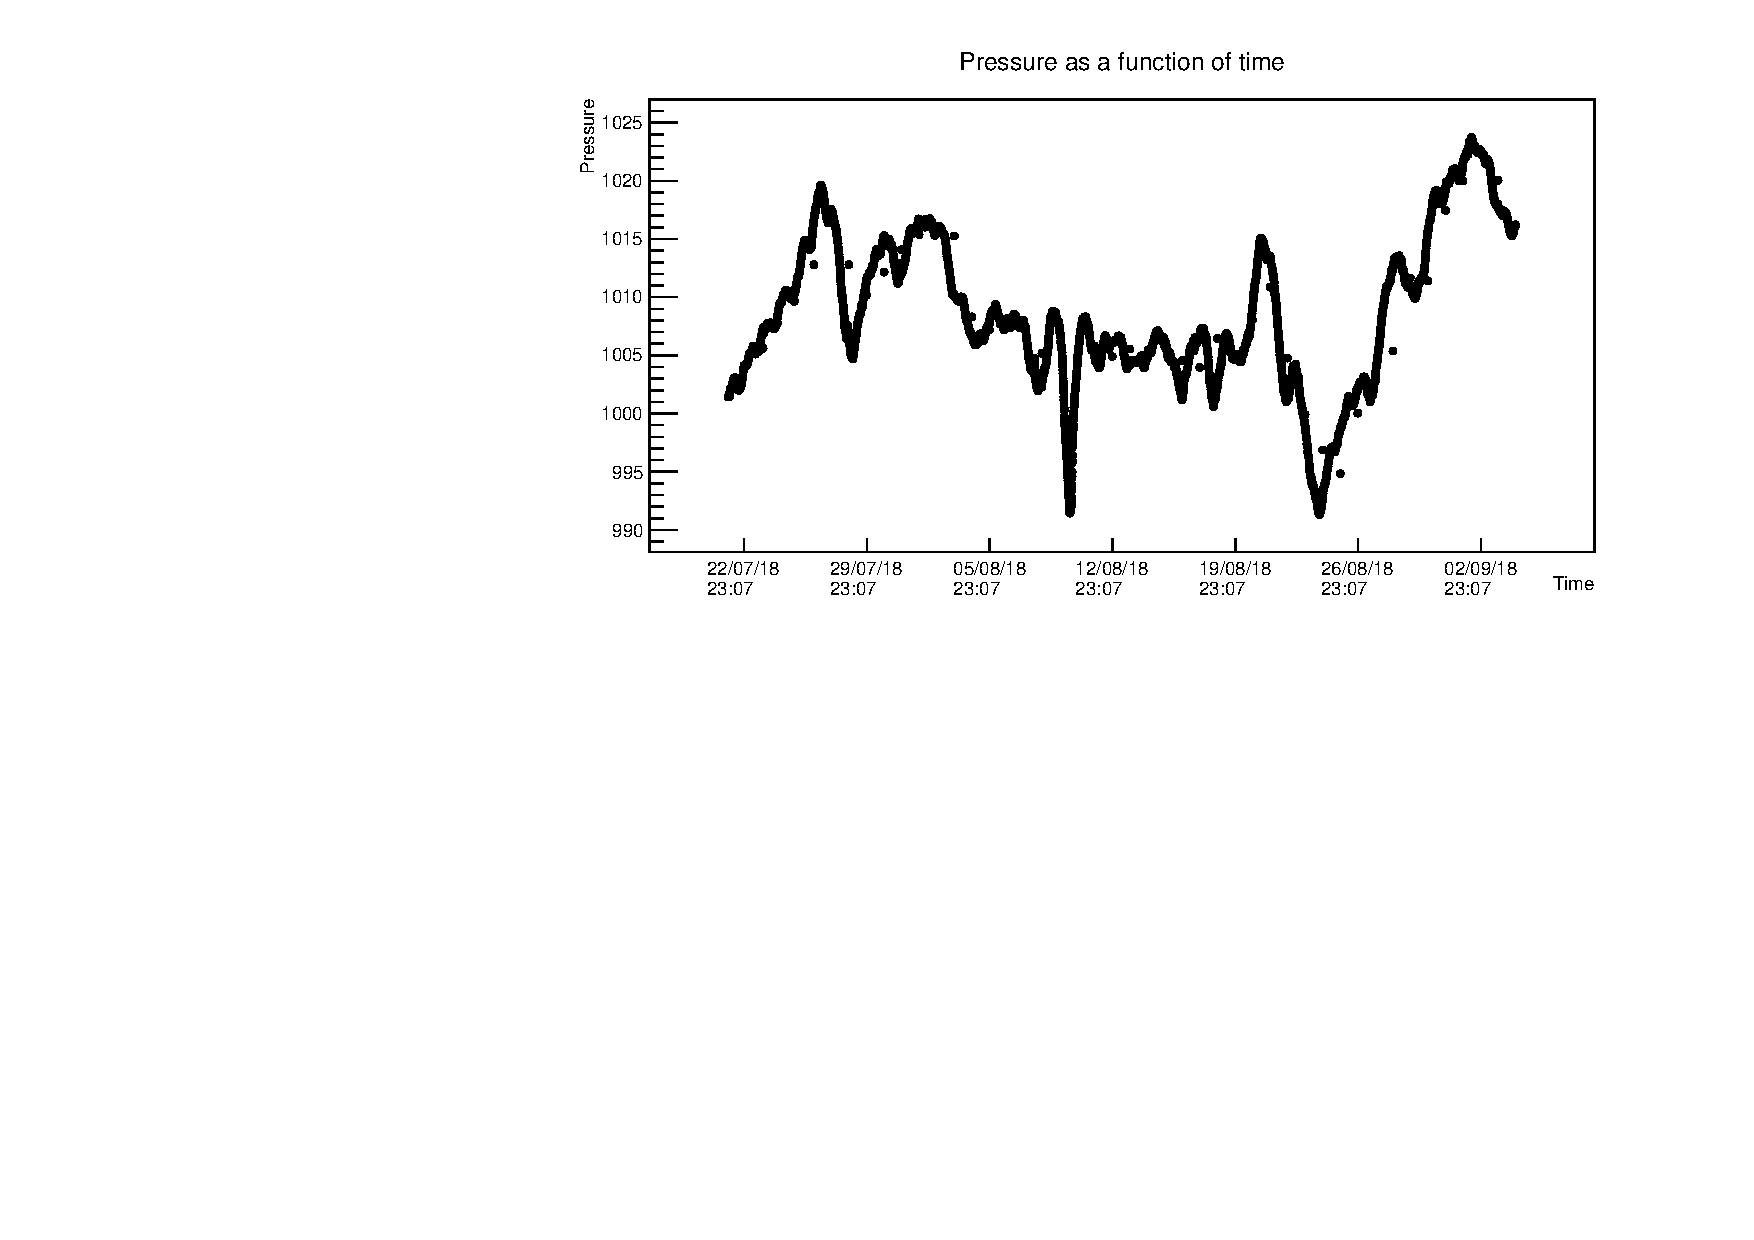
\includegraphics[width=\textwidth]{../data/plots/POLA-02/pressure_POLA-02.pdf}
		\caption{POLA-02}
		\label{fig:pressure_POLA-02}
	\end{subfigure}%
	\begin{subfigure}[b]{0.6\textwidth}
	\centering
		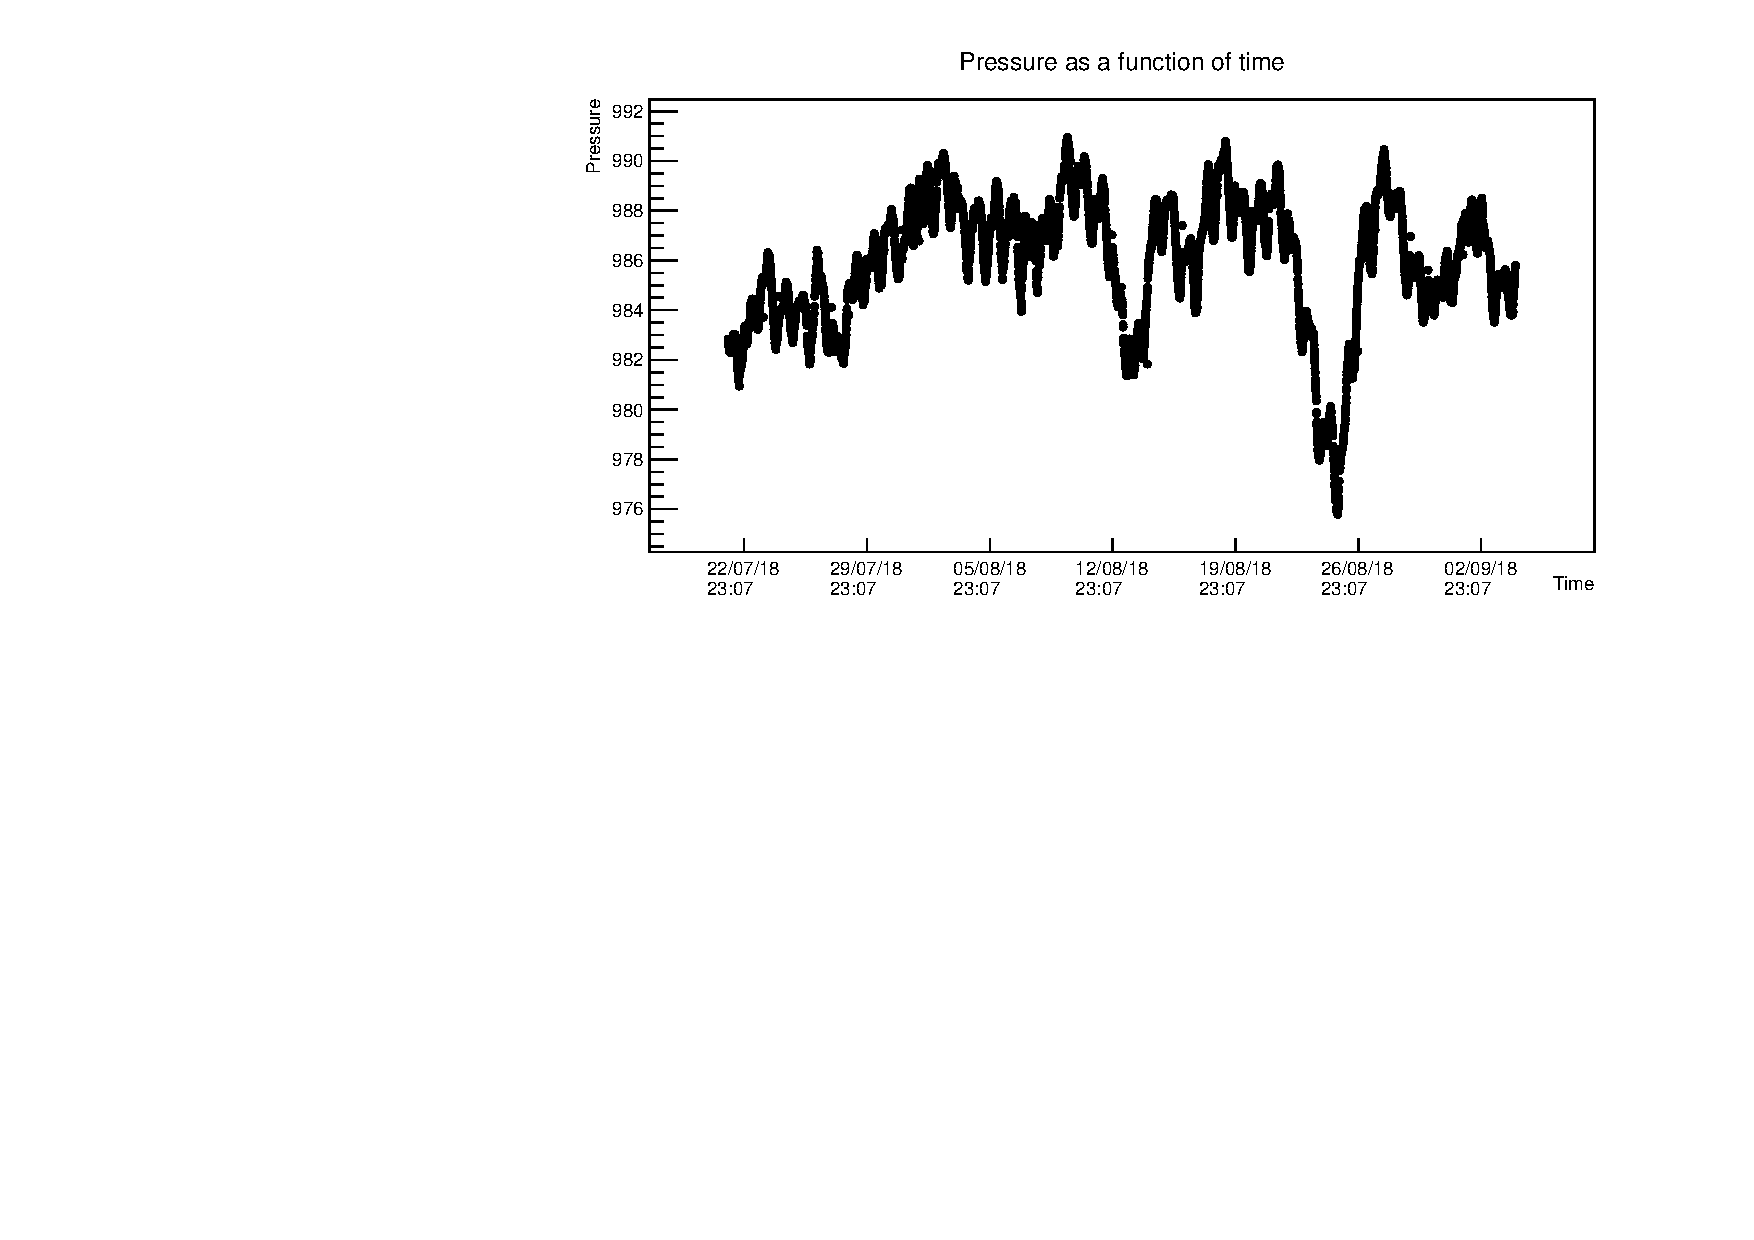
\includegraphics[width=\textwidth]{../data/plots/POLA-03/pressure_POLA-03.pdf}
		\caption{POLA-03}
		\label{fig:pressure_POLA-03}
	\end{subfigure}
	\caption{Barometric pressure each detector is subject to dependent on elevation above sea level.}
	\label{fig:pressure}
\end{figure}


\printbibliography


\end{document}









